\section{Satellite galaxies around a massive spiral}

\subsection{Exercise a}
\lstinputlisting{Integration.py}
\lstinputlisting{Exercise1abc.py}

For the first exercise, we will integrate Function 1 in order to find A such that the function is normalized. As the integral is a volume integral, we have to rewrite it to get to a 1D integral. This is Equation \ref{eq:integral}. 

\begin{equation}\label{eq:integral}
    \int\int\int n(x) dV = \int dx\ n(x)\cdot 4\pi \cdot x^2
\end{equation}

Now we have rewritten the integral, we will apply the algorithm of Romberg to find the result of the integral with the bounds 1e-4 and 5. By dividing 1 by the result of the integral, we will find the normalization factor A. This factor is calculated to be: 
\lstinputlisting{exercise1a.txt}

\subsection{Exercise b}
For subquestion B, we have to sample from this probability distribution, which we will do with rejection sampling. The first step of this is to write a random number generator (RNG). The RNG we will use is based on both XOR and Multiply with Carry. We first calculate a random number based on a seed. This seed is the current time, defined by time.time(). After a random number is generated with this seed, we will save the random number as a state for the calculation of the next random number. These states are saved for both XOR and Multiply with Carry separately. After this, both random numbers are combined to get the final random number. The following equation is used to define an upper and lower limit for the RNG. 

\begin{equation}
    U(a,b) = a + (b - a) U(0,1)
\end{equation}
where a is the minimum value, b the maximum value and U a uniform distribution.

Now we have the random number generator, we can start sampling. As said, this will be done with rejection sampling. We generate a number between xmin and xmax and a random number between 0 and the maximum of the probability distribution. Next, we calculate the value of the probability at the generated x and compare this with the generated y. If the generated y is lower than the probability distribution, the sample is accepted, and otherwise it is rejected. We continue with this till we have 10,000 accepted samples. The samples are plotted in a histogram along with the analytical probability distribution. This is shown in Figure \ref{fig:1b}.

\begin{figure}[h!]
  \centering
  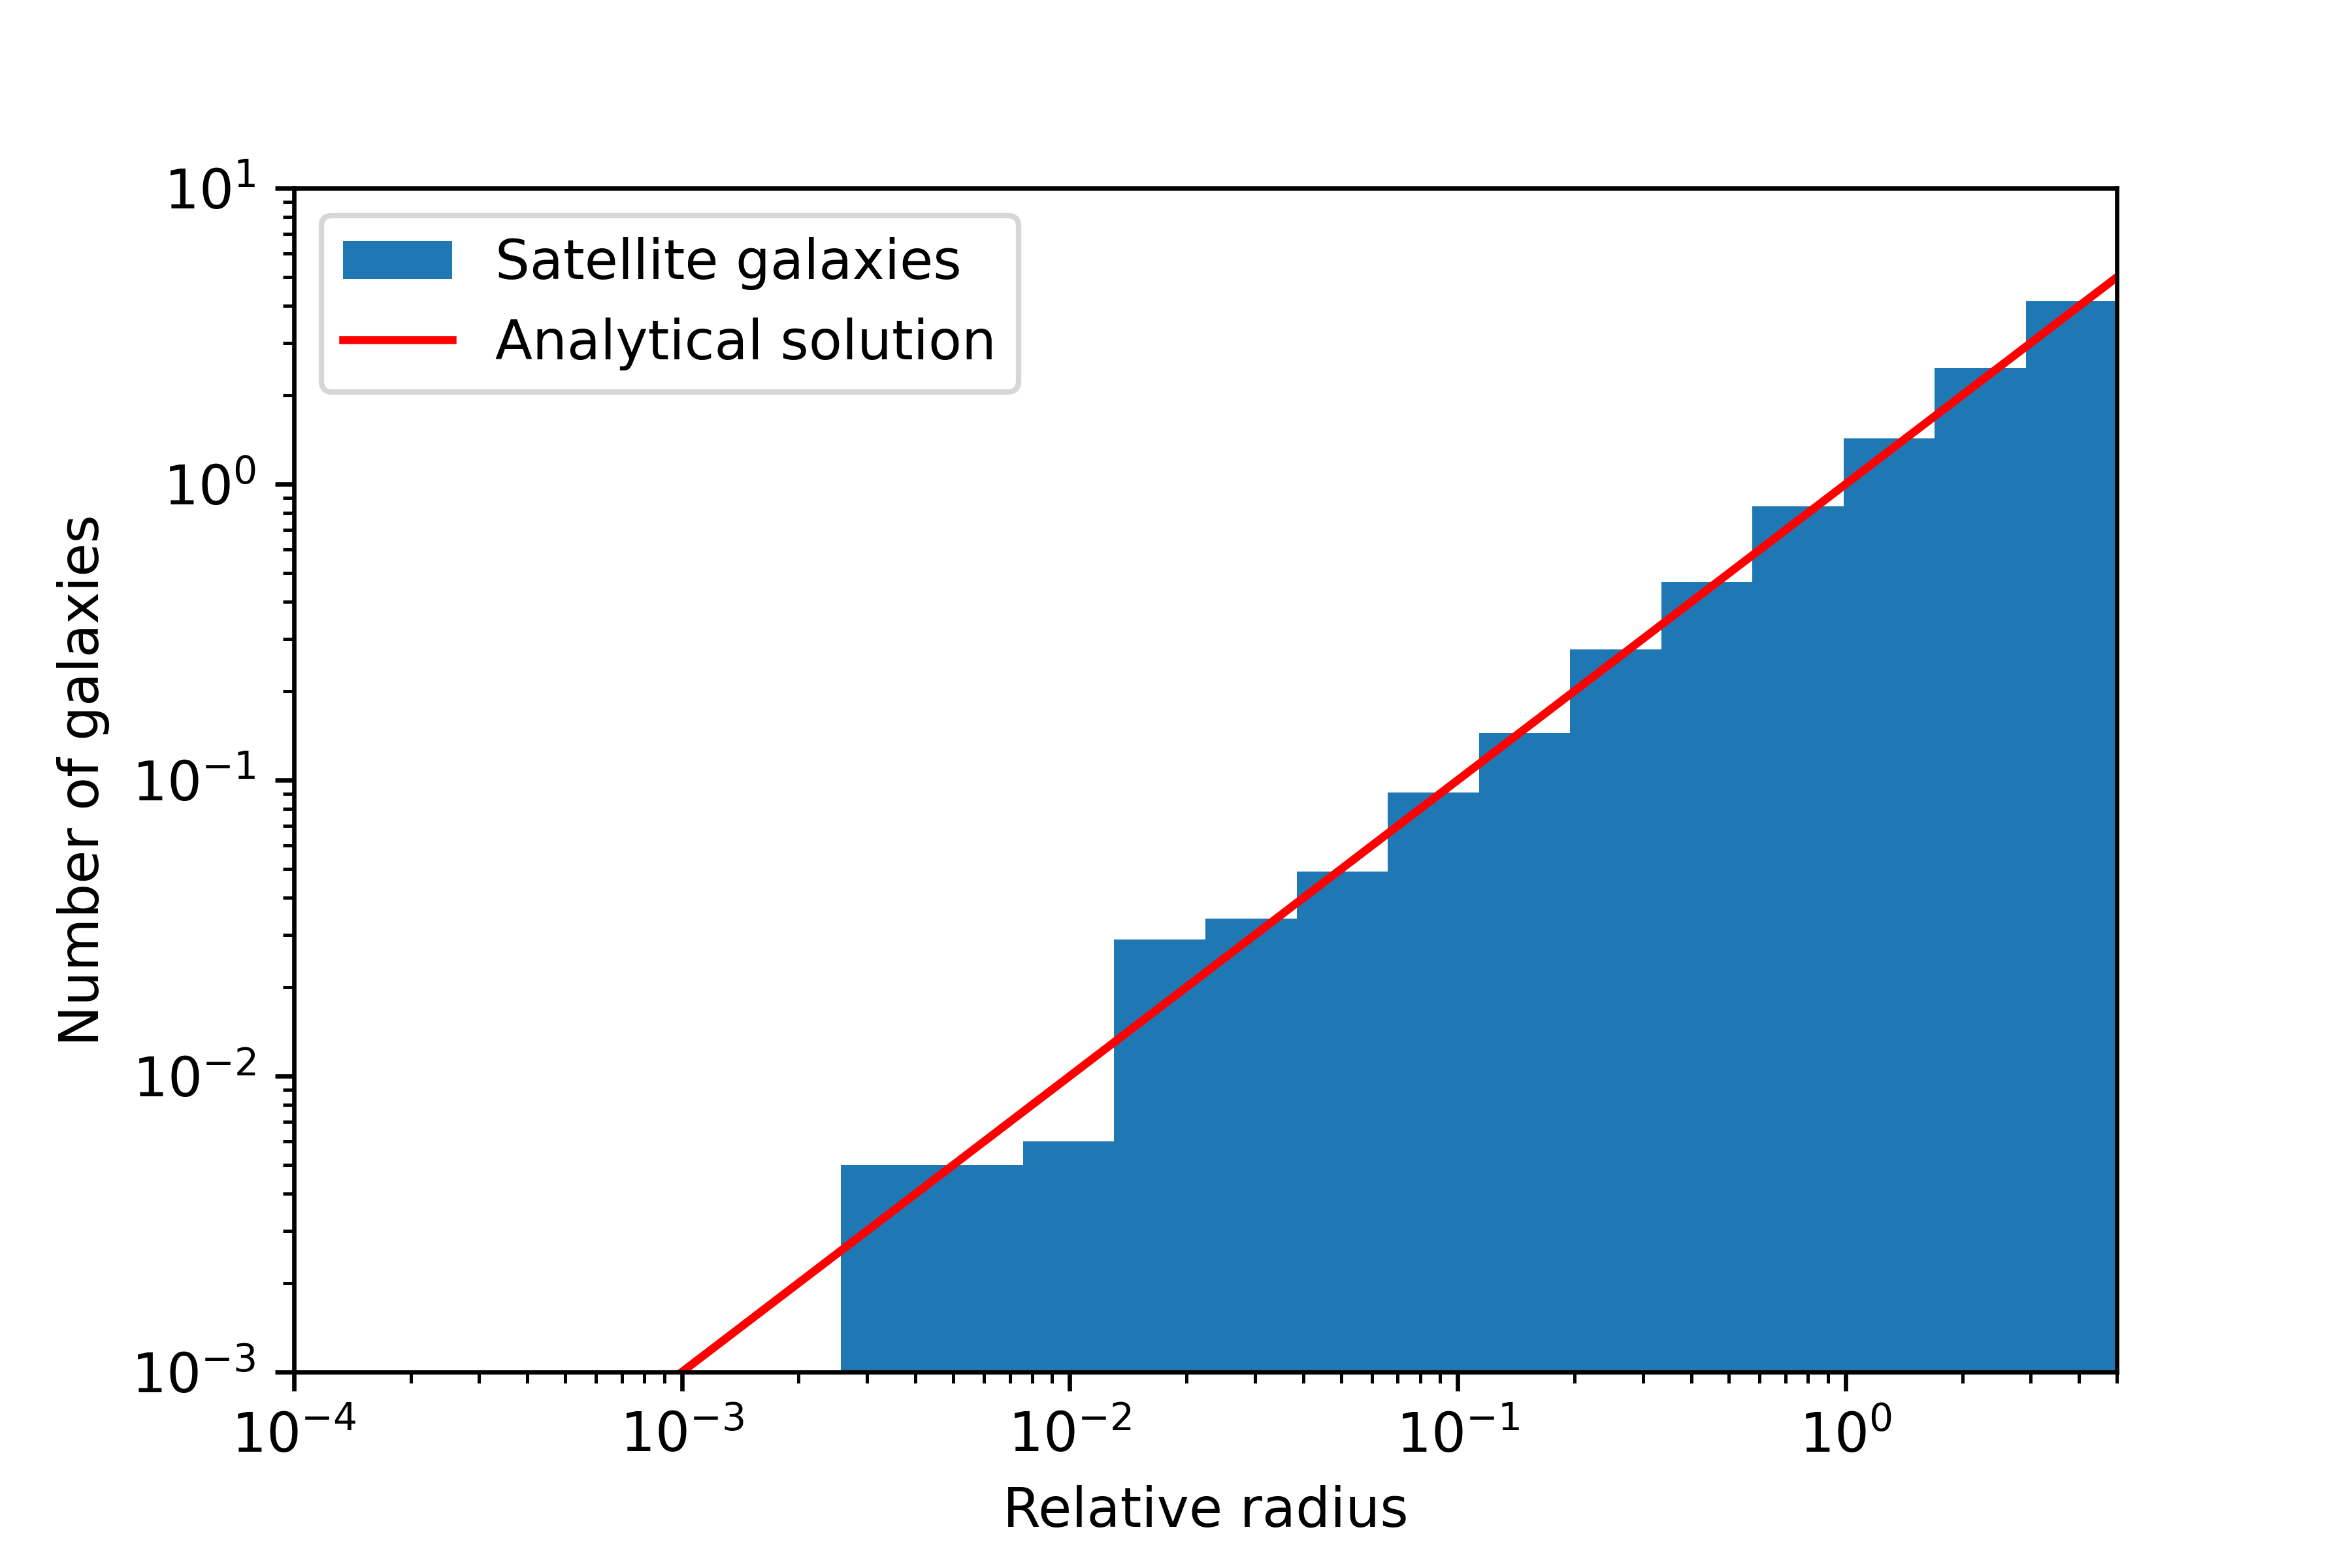
\includegraphics[width=0.9\linewidth]{my_solution_1b.png}
  \caption{The analytical probability distribution with a histogram of samples based on this probability distribution. Rejection sampling is used for creating the samples. For the lower radii, the samples are underrepresented, which might be caused by the low probability in that range of radii.}
  \label{fig:1b}
\end{figure}

\subsection{Exercise c}
In order to select 100 galaxies with equal probability, no double galaxies and without rejecting a draw, we will use a Fisher-Yates algorithm. This algorithm shuffles the array of galaxies and selects the first N galaxies. In this case N = 100. After that, we will use quicksort to sort the galaxies. The results of the sorting is shown in Figure \ref{fig:1c}.

\begin{figure}[h!]
  \centering
  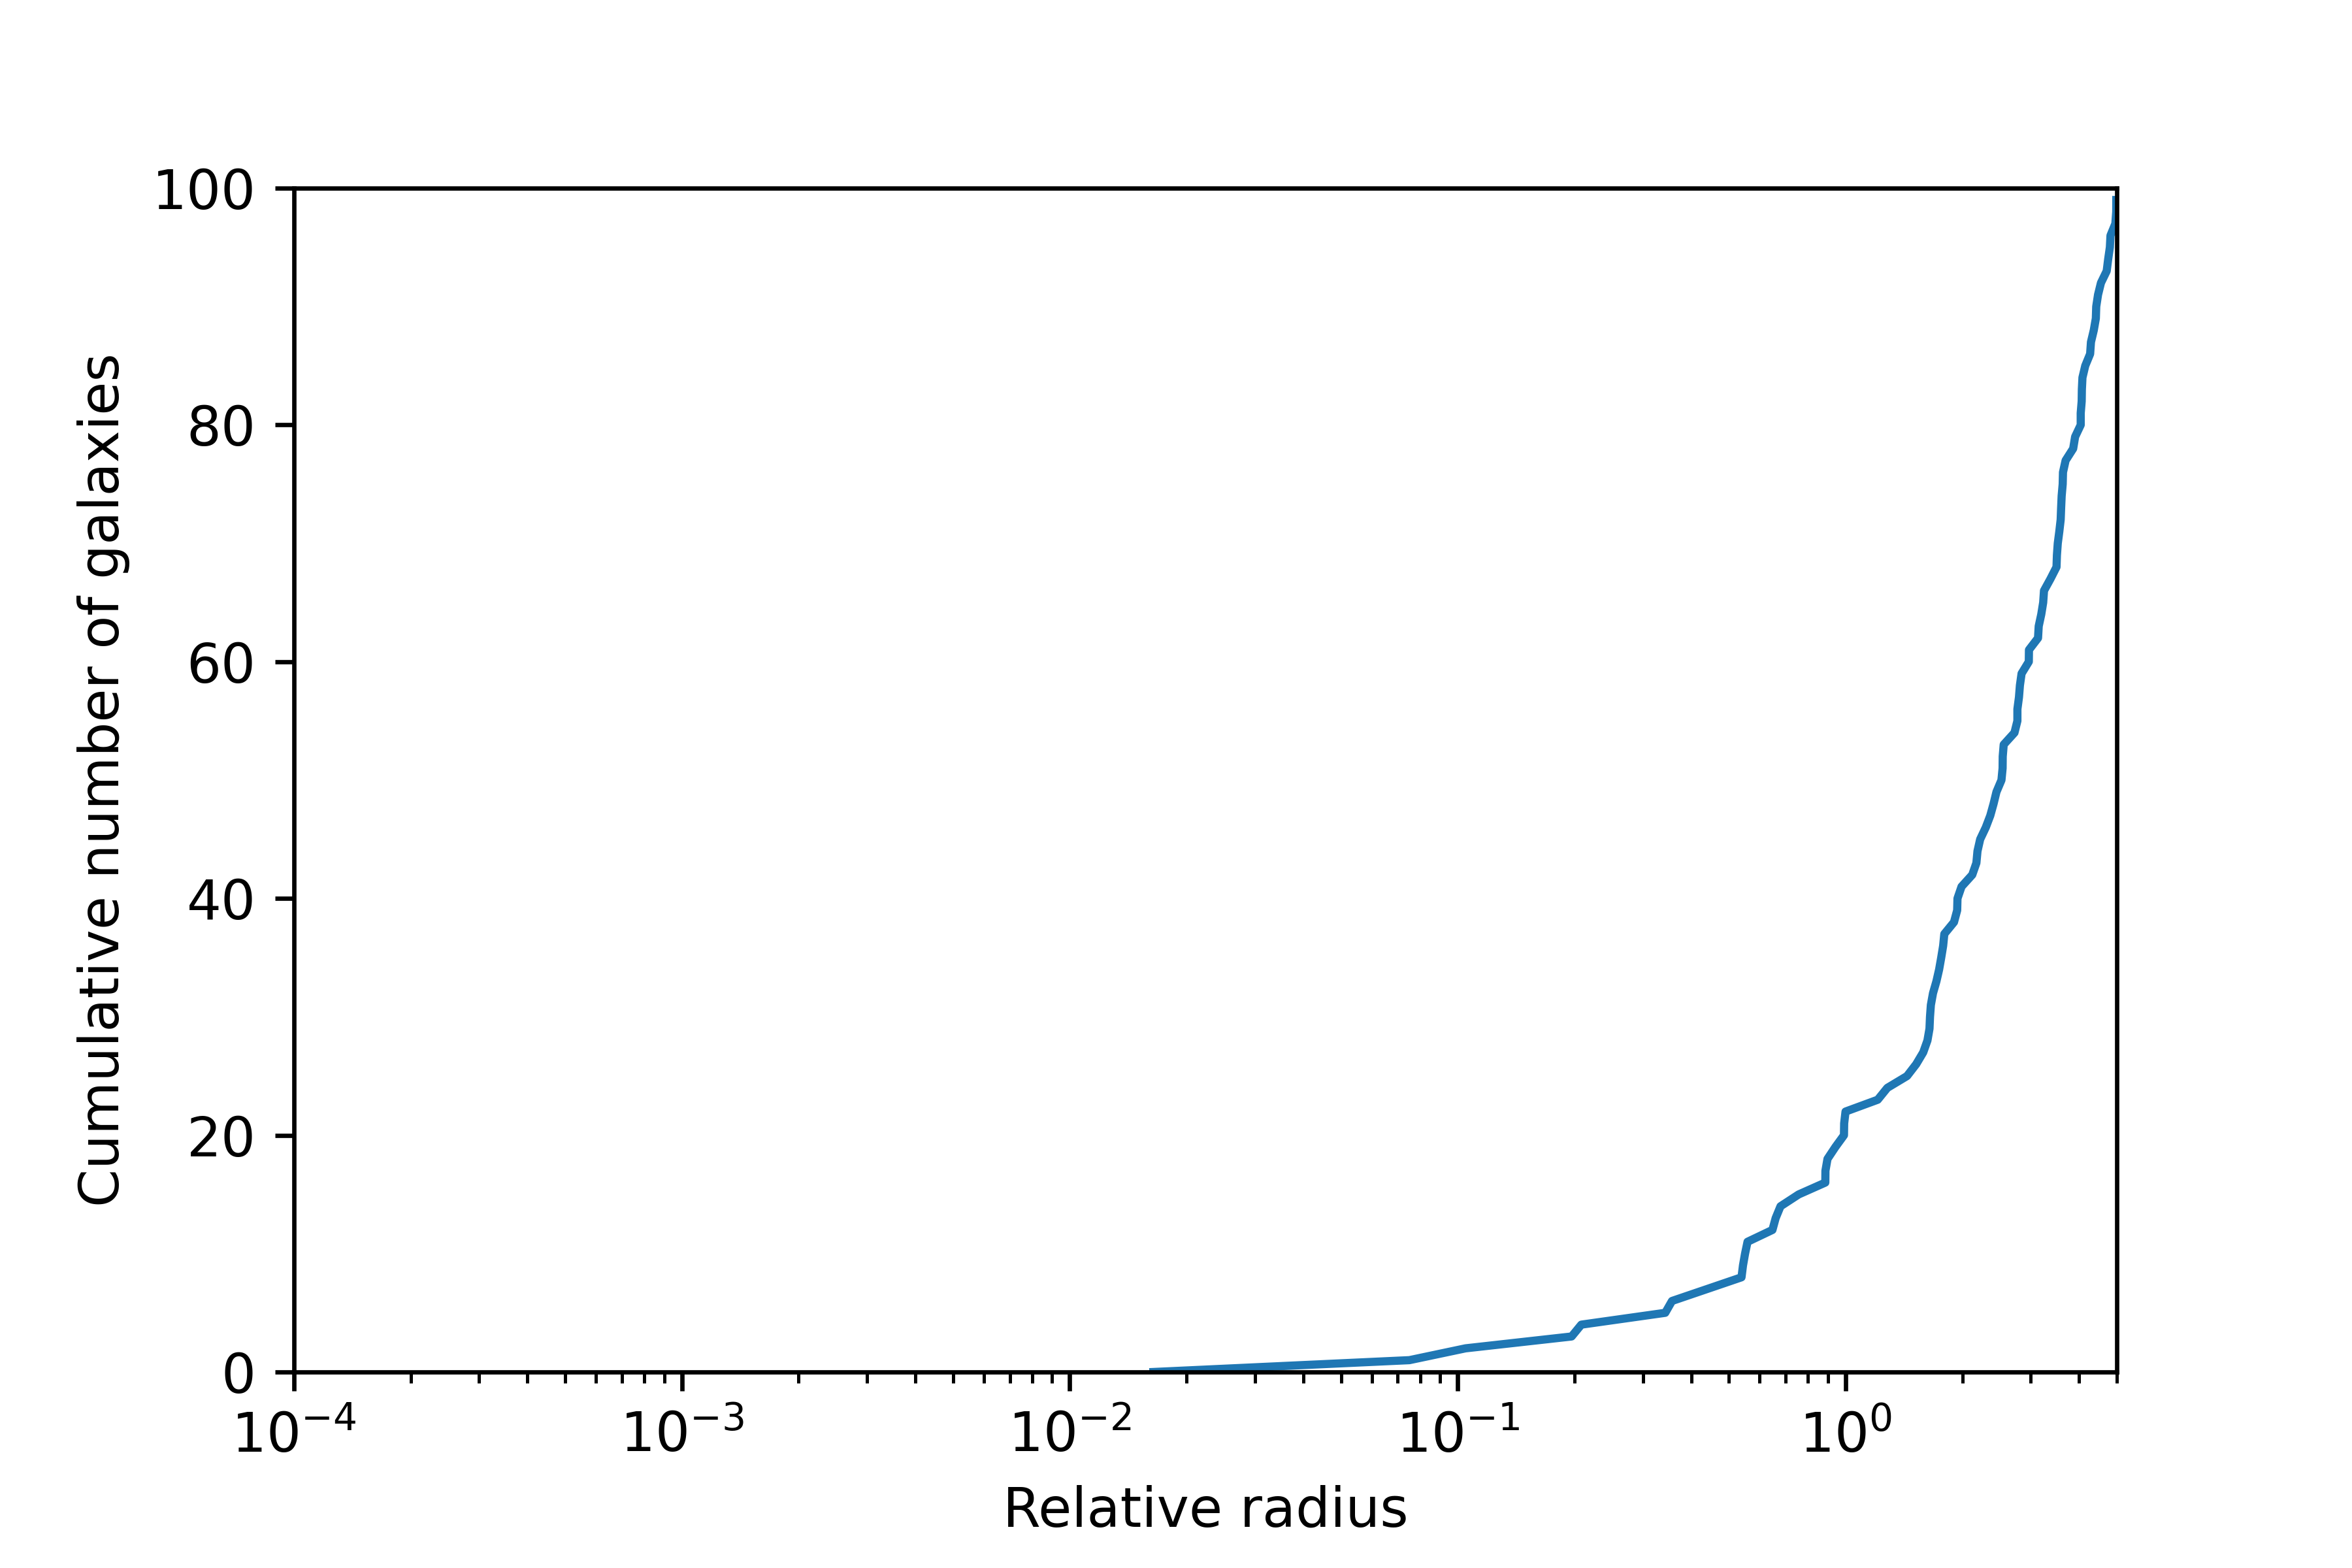
\includegraphics[width=0.9\linewidth]{my_solution_1c.png}
  \caption{The result of selecting and sorting 100 galaxies of the sample of 10,000 galaxies. In the figure, the line is increasing, which means the galaxies are correctly sorted.}
  \label{fig:1c}
\end{figure}

\subsection{Exercise d}
\lstinputlisting{Exercise1d.py}
Lastly, we want to differentiate n(x) at x = 1. This can be done both analytically and numerical. For the numerical solution, we will use a Ridder algorithm. This algorithm finds the numerical derivative, and stops when the error is growing. This is implemented to minimize the error between round-off and truncation errors. The result of both the analytical and numerical derivative is: 
\lstinputlisting{exercise1d.txt}



